\documentclass[]{article}
\usepackage{lmodern}
\usepackage{amssymb,amsmath}
\usepackage{ifxetex,ifluatex}
\usepackage{fixltx2e} % provides \textsubscript
\ifnum 0\ifxetex 1\fi\ifluatex 1\fi=0 % if pdftex
  \usepackage[T1]{fontenc}
  \usepackage[utf8]{inputenc}
\else % if luatex or xelatex
  \ifxetex
    \usepackage{mathspec}
  \else
    \usepackage{fontspec}
  \fi
  \defaultfontfeatures{Ligatures=TeX,Scale=MatchLowercase}
\fi
% use upquote if available, for straight quotes in verbatim environments
\IfFileExists{upquote.sty}{\usepackage{upquote}}{}
% use microtype if available
\IfFileExists{microtype.sty}{%
\usepackage{microtype}
\UseMicrotypeSet[protrusion]{basicmath} % disable protrusion for tt fonts
}{}
\usepackage[margin=1in]{geometry}
\usepackage{hyperref}
\hypersetup{unicode=true,
            pdftitle={Concept note: additional models},
            pdfborder={0 0 0},
            breaklinks=true}
\urlstyle{same}  % don't use monospace font for urls
\usepackage{graphicx,grffile}
\makeatletter
\def\maxwidth{\ifdim\Gin@nat@width>\linewidth\linewidth\else\Gin@nat@width\fi}
\def\maxheight{\ifdim\Gin@nat@height>\textheight\textheight\else\Gin@nat@height\fi}
\makeatother
% Scale images if necessary, so that they will not overflow the page
% margins by default, and it is still possible to overwrite the defaults
% using explicit options in \includegraphics[width, height, ...]{}
\setkeys{Gin}{width=\maxwidth,height=\maxheight,keepaspectratio}
\IfFileExists{parskip.sty}{%
\usepackage{parskip}
}{% else
\setlength{\parindent}{0pt}
\setlength{\parskip}{6pt plus 2pt minus 1pt}
}
\setlength{\emergencystretch}{3em}  % prevent overfull lines
\providecommand{\tightlist}{%
  \setlength{\itemsep}{0pt}\setlength{\parskip}{0pt}}
\setcounter{secnumdepth}{0}
% Redefines (sub)paragraphs to behave more like sections
\ifx\paragraph\undefined\else
\let\oldparagraph\paragraph
\renewcommand{\paragraph}[1]{\oldparagraph{#1}\mbox{}}
\fi
\ifx\subparagraph\undefined\else
\let\oldsubparagraph\subparagraph
\renewcommand{\subparagraph}[1]{\oldsubparagraph{#1}\mbox{}}
\fi

%%% Use protect on footnotes to avoid problems with footnotes in titles
\let\rmarkdownfootnote\footnote%
\def\footnote{\protect\rmarkdownfootnote}

%%% Change title format to be more compact
\usepackage{titling}

% Create subtitle command for use in maketitle
\newcommand{\subtitle}[1]{
  \posttitle{
    \begin{center}\large#1\end{center}
    }
}

\setlength{\droptitle}{-2em}
  \title{Concept note: additional models}
  \pretitle{\vspace{\droptitle}\centering\huge}
  \posttitle{\par}
\subtitle{Pradhan, Sicuri, Brew}
  \author{}
  \preauthor{}\postauthor{}
  \date{}
  \predate{}\postdate{}

\pagenumbering{gobble}
\usepackage{longtable}
\usepackage[utf8]{inputenc}
\usepackage{changepage}
\usepackage{graphicx}
\usepackage{multicol}
\usepackage{geometry}
\usepackage{fancyhdr}
\usepackage{color}
\usepackage{colortbl}
\usepackage{color}
\usepackage{hyperref}
% Font
\usepackage{fontspec}
\setmainfont{Swift-Regular_43151.ttf}
\setsansfont[BoldFont={Swift-Bold_43130.ttf}]{Swift-Regular_43151.ttf}
% \setmonofont{Swift-Regular_43151.ttf}
\renewcommand{\familydefault}{\sfdefault}
% \usepackage{fontspec}
% \setmainfont{Lato-Regular.ttf}
% \setsansfont[BoldFont={Lato-Bold.ttf}]{Lato-Regular.ttf}
% \renewcommand{\familydefault}{\sfdefault}

\def\changemargin#1#2{\list{}{\rightmargin#2\leftmargin#1}\item[]}
\let\endchangemargin=\endlist
\renewcommand{\rmdefault}{ppl}

\usepackage{multicol}
\usepackage{hyperref}
\usepackage{geometry}
\usepackage{lipsum}

\usepackage{longtable}


\usepackage{float}
\floatplacement{figure}{H}

% \usepackage{todonotes} % for side notes
% \usepackage[colorinlistoftodos]{todonotes} % for side notes

\usepackage{xargs}                      % Use more than one optional parameter in a new commands
\usepackage[dvipsnames, table]{xcolor}  % Coloured text etc.
% 
\usepackage[colorinlistoftodos,prependcaption,textsize=tiny]{todonotes}
\newcommandx{\unsure}[2][1=]{\todo[linecolor=red,backgroundcolor=red!25,bordercolor=red,#1]{#2}}
\newcommandx{\change}[2][1=]{\todo[linecolor=blue,backgroundcolor=blue!25,bordercolor=blue,#1]{#2}}
\newcommandx{\info}[2][1=]{\todo[linecolor=OliveGreen,backgroundcolor=OliveGreen!25,bordercolor=OliveGreen,#1]{#2}}
\newcommandx{\improvement}[2][1=]{\todo[linecolor=Plum,backgroundcolor=Plum!25,bordercolor=Plum,#1]{#2}}
\newcommandx{\thiswillnotshow}[2][1=]{\todo[disable,#1]{#2}}
\usepackage{lmodern}
\usepackage{fancyhdr} % Headers and footers
\pagestyle{fancy} % All pages have headers and footers
\fancyhead{} % Blank out the default header
\fancyfoot{} % Blank out the default footer
\fancyhead[C]{Return on investment of private sector malaria control at a large sugar facility in Southern Mozambique}
\renewcommand{\thefootnote}{\fnsymbol{footnote}}

\newcommand{\footremember}[2]{%
    \footnote{#2}
    \newcounter{#1}
    \setcounter{#1}{\value{footnote}}%
}
\newcommand{\footrecall}[1]{%
    \footnotemark[\value{#1}]%
}

\def\changemargin#1#2{\list{}{\rightmargin#2\leftmargin#1}\item[]}
\let\endchangemargin=\endlist

\widowpenalties 1 150

\makeatletter
\renewcommand\footnotesize{%
   \@setfontsize\footnotesize\@ixpt{11}%
   \abovedisplayskip 8\p@ \@plus2\p@ \@minus4\p@
   \abovedisplayshortskip \z@ \@plus\p@
   \belowdisplayshortskip 4\p@ \@plus2\p@ \@minus2\p@
   \def\@listi{\leftmargin\leftmargini
               \topsep 4\p@ \@plus2\p@ \@minus2\p@
               \parsep 2\p@ \@plus\p@ \@minus\p@
               \itemsep \parsep}%
   \belowdisplayskip \abovedisplayskip
}
\makeatother

\DeclareTextCommandDefault{\nobreakspace}{\leavevmode\nobreak\ }
\usepackage{booktabs}
\usepackage{longtable}
\usepackage{array}
\usepackage{multirow}
\usepackage[table]{xcolor}
\usepackage{wrapfig}
\usepackage{float}
\usepackage{colortbl}
\usepackage{pdflscape}
\usepackage{tabu}
\usepackage{threeparttable}

\begin{document}
\maketitle

\begin{center}
\begin{large}

A few different approaches to modeling absenteeism in the Maragra data

\end{large}
\end{center}

\vspace{5mm}

\begin{center}
\textbf{Overview}  
\end{center}

\vspace{5mm}

\begin{center}
\begin{changemargin}{3cm}{3cm} 

This document contains methods and basic results for a few different modeling approaches, following a conversation and write-up with Menno Pradhan in May 2018. The purpose of this document is to make explicit the current models we have implemented, and some issues with them.

\end{changemargin}
\end{center}

\vspace{20mm}

\noindent\fbox{%
    \parbox{\textwidth}{%
        \subsection*{Main points}
        \begin{itemize}
          \item I have implemented Menno's suggestions for more simple models.
          \item The simplest models show no overall effect from IRS when not accounting for malaria season
          \item I believe that the lack of an effect is due to seasonality's presence in the model as a fixed (additive) effect, rather than as an interaction with IRS
        \end{itemize}
        \vspace{2mm}
    }%
}

\vfill
\null

\subsection*{Desinataires}

\textbf{Elisa Sicuri; Menno Pradhan}

\vspace{3mm}

\newpage

\section{The current approach}\label{the-current-approach}

In the current draft of the paper
(\href{https://docs.google.com/document/d/1bUWRBCgVcgjSPHchIQxiTG8Vwv5hV1GLU4Tlu386sWA/edit#}{HERE}
), the model formula is:

\[
\hat{Y_{it}} = \hat{\beta}_{0} +  \hat{\beta}_{1}\text{Season}_{t} * IRS_{it} + \hat{\beta}_2{RainyDay_{t}} + \hat{\beta}_3{Herd_{it}} +  \alpha_i + \delta_t + \upsilon_{it}
\]

In R, using the \texttt{felm} library, this is written as follows:

\begin{verbatim}
felm(formula = absent ~ season * months_since + rainy_day + herd | 
    oracle_number + malaria_year | 0 | 0, data = these_data)
\end{verbatim}

The above notation shows \texttt{absent} (binary 1,0) as a function of
the interaction of binary \texttt{season} (high vs.~low) and binary
\texttt{months\_since} (before vs.~after) plus binary
\texttt{rainy\_day} (whether or not it rained on the particular day)
plus continuous numeric \texttt{herd} (ie, the protection afforded by
others) plus fixed effects for both the worker (\texttt{oracle\_number})
and the year (\texttt{malaria\_year}). \(\alpha_i\) represents the time
invariant worker fixed effects, and \(\delta_i\) represents the fixed
effect of the particular malaria season. \(\upsilon\) is the error term.
This model is run separately for the 4 different worker groups, yielding
the following results:

\begin{longtable}[t]{ll}
\caption{\label{tab:unnamed-chunk-4}All absenteeism with herd immunity: model results}\\
\toprule
Term & Estimate\\
\midrule
\endfirsthead
\caption[]{All absenteeism with herd immunity: model results \textit{(continued)}}\\
\toprule
Term & Estimate\\
\midrule
\endhead
\
\endfoot
\bottomrule
\endlastfoot
\addlinespace[1.5em]
\multicolumn{2}{l}{\textbf{Permanent field worker}}\\
\hspace{1em}Malaria season & 0.034 (P<0.001)\\
\hspace{1em}IRS status=After & 0.035 (P<0.001)\\
\hspace{1em}Rainy day & 0.027 (P<0.001)\\
\hspace{1em}Herd protection & 0 (P=0.001)\\
\hspace{1em}Malaria season:IRS status=After & -0.04 (P<0.001)\\
\addlinespace[1.5em]
\multicolumn{2}{l}{\textbf{Permanent not field worker}}\\
\hspace{1em}Malaria season & 0.009 (P<0.001)\\
\hspace{1em}IRS status=After & 0.005 (P=0.054)\\
\hspace{1em}Rainy day & 0.045 (P<0.001)\\
\hspace{1em}Herd protection & 0 (P<0.001)\\
\hspace{1em}Malaria season:IRS status=After & -0.015 (P<0.001)\\
\addlinespace[1.5em]
\multicolumn{2}{l}{\textbf{Temporary field worker}}\\
\hspace{1em}Malaria season & -0.003 (P<0.001)\\
\hspace{1em}IRS status=After & 0.001 (P=0.127)\\
\hspace{1em}Rainy day & 0.001 (P=0.032)\\
\hspace{1em}Herd protection & 0 (P=0.242)\\
\hspace{1em}Malaria season:IRS status=After & 0.001 (P=0.274)\\
\addlinespace[1.5em]
\multicolumn{2}{l}{\textbf{Temporary not field worker}}\\
\hspace{1em}Malaria season & 0.033 (P<0.001)\\
\hspace{1em}IRS status=After & -0.007 (P=0.313)\\
\hspace{1em}Rainy day & 0.002 (P=0.409)\\
\hspace{1em}Herd protection & 0 (P=0.974)\\
\hspace{1em}Malaria season:IRS status=After & -0.007 (P=0.405)\\*
\end{longtable}

In the above, ``after'' IRS application (ie, the 6 months following IRS)
is associated with a significant reduction in absenteeism for both kinds
of permanent workers, and does not have a signficiant association with a
change in absenteeism for both kinds of temporary workers.

\section{Suggested changes from
Menno}\label{suggested-changes-from-menno}

Menno sent a write-up on May 17th (see email with subject ``suggestions
for models'') with some proposed changes to how we model absenteeism.
What follows is an implementation of those suggestions.

\subsection{Model A (without
seasonality)}\label{model-a-without-seasonality}

The below is a characterization of the approach Menno suggested:

\begin{itemize}
\tightlist
\item
  We use monthly instead of daily data (modeling a percentage
  absenteeism rate rather than a binary).
\item
  We use fixed effects for year-month combination.
\item
  We don't explicitly model for malaria season.
\item
  We don't have any interaction terms.
\item
  We use dummies for months since IRS.
\item
  We use the most recent spraying as the time since IRS (ie, if 5 months
  ago, and 1 month ago, then the dummy is applied for 1 month ago but
  not 5 months ago).
\end{itemize}

Using this approach, our panel data looks like this:

\begin{verbatim}
# A tibble: 6 x 6
  oracle_number group            year_month absent  days months_since_men~
  <chr>         <chr>            <chr>       <dbl> <int> <fct>            
1 X045753       Temporary field~ 2015_10       0      13 01               
2 X040254       Temporary field~ 2016_9        0      30 01               
3 X040343       Temporary field~ 2014_6        0      30 03               
4 PF02071       Temporary not f~ 2015_3       80.6    31 06               
5 PA00795       Permanent field~ 2013_3       67.7    31 02               
6 PF00699       Permanent not f~ 2016_3        0      31 06               
\end{verbatim}

The model formula was described in Menno's email.

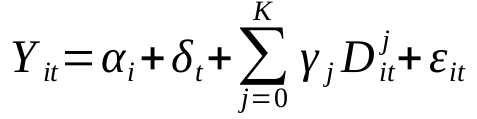
\includegraphics{images/menno}{[}width=3cm{]}

Which translates into R as:

\begin{verbatim}
felm(formula = absent ~ months_since_menno | oracle_number + 
    year_month | 0 | 0, data = these_data)
\end{verbatim}

Note that the \texttt{months\_since\_menno} variable has the following
categories, and is treated as a ``wide'' dummy by the software in
modeling:

\begin{verbatim}
[1] "Before" "01"     "02"     "03"     "04"     "05"     "06"    
\end{verbatim}

The results of this model look like this:

\begin{longtable}[t]{ll}
\caption{\label{tab:unnamed-chunk-8}Simple models with year-month fixed effects}\\
\toprule
Term & Estimate\\
\midrule
\endfirsthead
\caption[]{Simple models with year-month fixed effects \textit{(continued)}}\\
\toprule
Term & Estimate\\
\midrule
\endhead
\
\endfoot
\bottomrule
\endlastfoot
\addlinespace[1.5em]
\multicolumn{2}{l}{\textbf{Permanent field worker}}\\
\hspace{1em}IRS status=\_menno01 & 1.425 (P=0.446)\\
\hspace{1em}IRS status=\_menno02 & 3.603 (P=0.066)\\
\hspace{1em}IRS status=\_menno03 & 2.049 (P=0.297)\\
\hspace{1em}IRS status=\_menno04 & 1.357 (P=0.491)\\
\hspace{1em}IRS status=\_menno05 & 1.351 (P=0.498)\\
\hspace{1em}IRS status=\_menno06 & 3.358 (P=0.106)\\
\addlinespace[1.5em]
\multicolumn{2}{l}{\textbf{Permanent not field worker}}\\
\hspace{1em}IRS status=\_menno01 & -0.022 (P=0.982)\\
\hspace{1em}IRS status=\_menno02 & 0.255 (P=0.805)\\
\hspace{1em}IRS status=\_menno03 & 1.803 (P=0.085)\\
\hspace{1em}IRS status=\_menno04 & -0.87 (P=0.406)\\
\hspace{1em}IRS status=\_menno05 & 0.144 (P=0.894)\\
\hspace{1em}IRS status=\_menno06 & 0.073 (P=0.947)\\
\addlinespace[1.5em]
\multicolumn{2}{l}{\textbf{Temporary field worker}}\\
\hspace{1em}IRS status=\_menno01 & -0.333 (P=0.261)\\
\hspace{1em}IRS status=\_menno02 & -0.058 (P=0.847)\\
\hspace{1em}IRS status=\_menno03 & -0.378 (P=0.215)\\
\hspace{1em}IRS status=\_menno04 & 0.01 (P=0.973)\\
\hspace{1em}IRS status=\_menno05 & 0.075 (P=0.797)\\
\hspace{1em}IRS status=\_menno06 & 0.41 (P=0.17)\\
\addlinespace[1.5em]
\multicolumn{2}{l}{\textbf{Temporary not field worker}}\\
\hspace{1em}IRS status=\_menno01 & 0.08 (P=0.979)\\
\hspace{1em}IRS status=\_menno02 & 2.989 (P=0.35)\\
\hspace{1em}IRS status=\_menno03 & -4.094 (P=0.167)\\
\hspace{1em}IRS status=\_menno04 & -2.276 (P=0.449)\\
\hspace{1em}IRS status=\_menno05 & -2.259 (P=0.464)\\
\hspace{1em}IRS status=\_menno06 & 2.409 (P=0.427)\\*
\end{longtable}

In the above, it is apparent that the effects of IRS appear to be either
(a) in the opposite direction as expected or (b) non-signficant. Here is
a visualization of IRS' apparent effect (relative to the ``Before''
period, which is the reference class). Were IRS effective, we would
expect the black line to be below 0 (the red line).

\begin{center}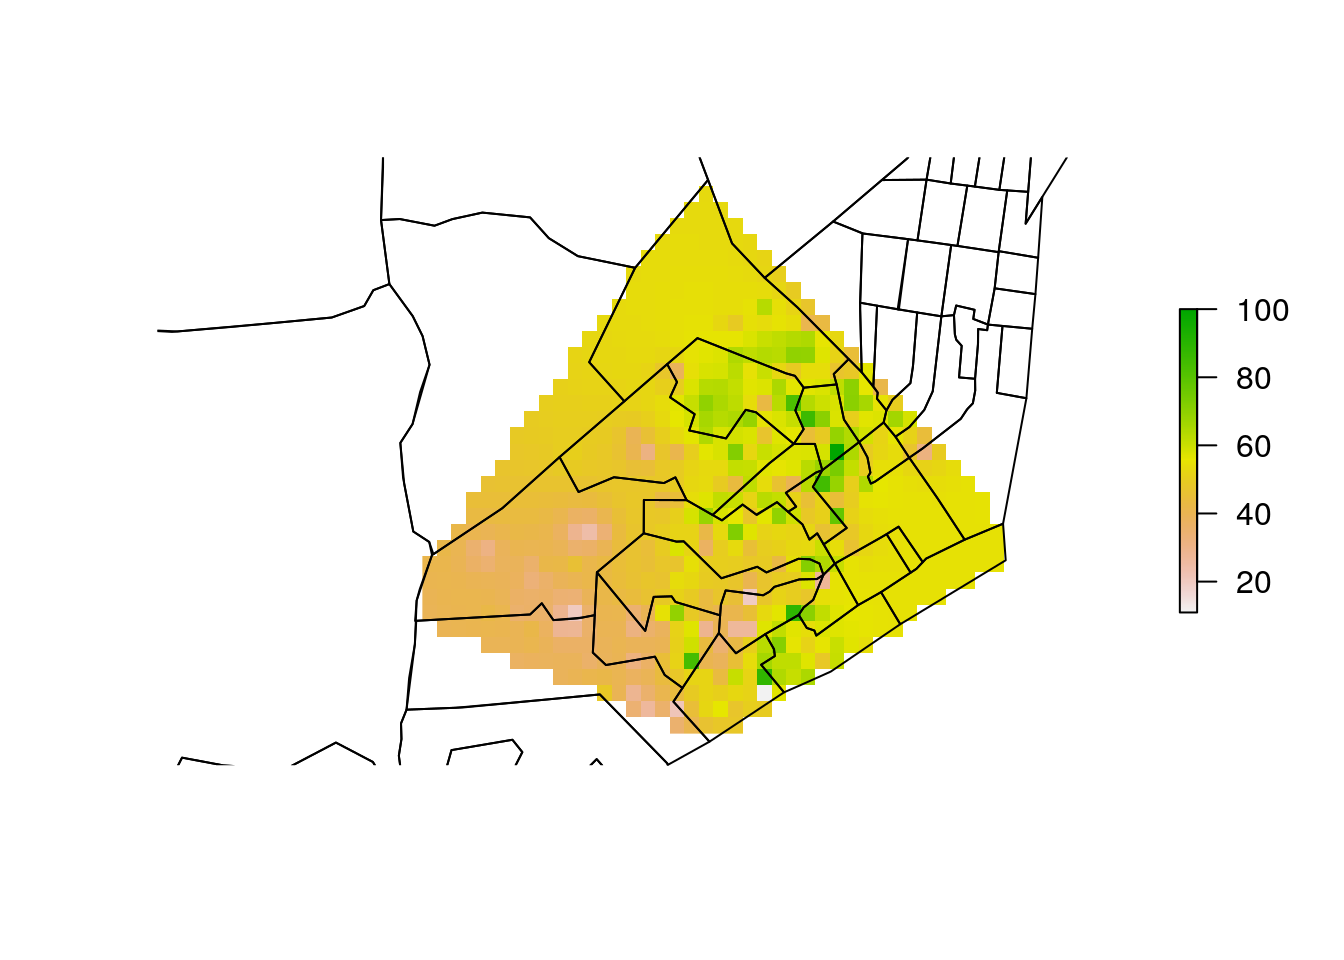
\includegraphics{menno_models_files/figure-latex/unnamed-chunk-9-1} \end{center}

What is going on here? Could it be that IRS has a positive (ie,
increases) impact on absenteeism? Let's look at the raw data, rather
than the coefficients. The below chart shows absenteeism (as a
percentage of the pre-IRS absenteeism average) for workers, broken down
by season (row) and worker type (column), with point size reflecting the
number of observations.

\begin{center}\includegraphics{menno_models_files/figure-latex/unnamed-chunk-10-1} \end{center}

In the above chart, two things stand out:

\begin{enumerate}
\def\labelenumi{\arabic{enumi}.}
\tightlist
\item
  Variability is greatest among temporary workers.
\item
  There appears to be a reduction in absenteeism post IRS for permanent
  workers \emph{during the malaria season}, but not during the
  non-malaria season
\end{enumerate}

So, perhaps controlling for year-month through fixed effects isn't
enough, since the effect of IRS \emph{interacts} with the season\ldots{}

\subsection{Model B (with seasonality)}\label{model-b-with-seasonality}

Using this approach, our panel data looks like this:

\begin{verbatim}
# A tibble: 6 x 7
  oracle_number group      year_month absent  days months_since_me~ season
  <chr>         <chr>      <chr>       <dbl> <int> <fct>            <fct> 
1 X037697       Temporary~ 2016_7       0       31 05               low   
2 PF01761       Permanent~ 2015_12      3.23    31 04               high  
3 X040726       Temporary~ 2015_5       3.23    31 02               high  
4 PF00774       Permanent~ 2014_6       3.33    30 04               low   
5 X043249       Temporary~ 2016_4       0       30 06               high  
6 X037700       Permanent~ 2013_2       0       27 02               high  
\end{verbatim}

Our new model specification (in R) is:

\begin{verbatim}
felm(formula = absent ~ months_since_menno * season | oracle_number + 
    year_month | 0 | 0, data = these_data)
\end{verbatim}

The results of this model look like this:

\begin{longtable}[t]{ll}
\caption{\label{tab:unnamed-chunk-13}Simple models with year-month fixed effects and seasonality-IRS interaction term}\\
\toprule
Term & Estimate\\
\midrule
\endfirsthead
\caption[]{Simple models with year-month fixed effects and seasonality-IRS interaction term \textit{(continued)}}\\
\toprule
Term & Estimate\\
\midrule
\endhead
\
\endfoot
\bottomrule
\endlastfoot
\addlinespace[1.5em]
\multicolumn{2}{l}{\textbf{Permanent field worker}}\\
\hspace{1em}IRS status=\_menno01 & 175.053 (P=0.532)\\
\hspace{1em}IRS status=\_menno02 & 457.807 (P=0.115)\\
\hspace{1em}IRS status=\_menno03 & 505.425 (P=0.061)\\
\hspace{1em}IRS status=\_menno04 & 233.373 (P=0.357)\\
\hspace{1em}IRS status=\_menno05 & 227.399 (P=0.372)\\
\hspace{1em}IRS status=\_menno06 & 425.265 (P=0.121)\\
\hspace{1em}Malaria season & 887.601 (P=0.703)\\
\hspace{1em}IRS status=\_menno01:Malaria season & -58.338 (P=0.872)\\
\hspace{1em}IRS status=\_menno02:Malaria season & -174.777 (P=0.642)\\
\hspace{1em}IRS status=\_menno03:Malaria season & -603.926 (P=0.105)\\
\hspace{1em}IRS status=\_menno04:Malaria season & -220.413 (P=0.56)\\
\hspace{1em}IRS status=\_menno05:Malaria season & -213.141 (P=0.582)\\
\hspace{1em}IRS status=\_menno06:Malaria season & -191.654 (P=0.633)\\
\addlinespace[1.5em]
\multicolumn{2}{l}{\textbf{Permanent not field worker}}\\
\hspace{1em}IRS status=\_menno01 & 39.635 (P=0.788)\\
\hspace{1em}IRS status=\_menno02 & 14.833 (P=0.919)\\
\hspace{1em}IRS status=\_menno03 & 114.878 (P=0.439)\\
\hspace{1em}IRS status=\_menno04 & 55.896 (P=0.694)\\
\hspace{1em}IRS status=\_menno05 & 93.301 (P=0.502)\\
\hspace{1em}IRS status=\_menno06 & 86.299 (P=0.556)\\
\hspace{1em}Malaria season & NaN (PNA)\\
\hspace{1em}IRS status=\_menno01:Malaria season & -72.876 (P=0.707)\\
\hspace{1em}IRS status=\_menno02:Malaria season & 23.995 (P=0.903)\\
\hspace{1em}IRS status=\_menno03:Malaria season & 127.34 (P=0.523)\\
\hspace{1em}IRS status=\_menno04:Malaria season & -296.411 (P=0.137)\\
\hspace{1em}IRS status=\_menno05:Malaria season & -185.639 (P=0.372)\\
\hspace{1em}IRS status=\_menno06:Malaria season & -171.932 (P=0.416)\\
\addlinespace[1.5em]
\multicolumn{2}{l}{\textbf{Temporary field worker}}\\
\hspace{1em}IRS status=\_menno01 & -35.174 (P=0.339)\\
\hspace{1em}IRS status=\_menno02 & -6.152 (P=0.869)\\
\hspace{1em}IRS status=\_menno03 & -12.472 (P=0.732)\\
\hspace{1em}IRS status=\_menno04 & 18.095 (P=0.611)\\
\hspace{1em}IRS status=\_menno05 & 33.497 (P=0.346)\\
\hspace{1em}IRS status=\_menno06 & 9.614 (P=0.816)\\
\hspace{1em}Malaria season & 44.327 (P=0.309)\\
\hspace{1em}IRS status=\_menno01:Malaria season & 8.557 (P=0.881)\\
\hspace{1em}IRS status=\_menno02:Malaria season & 3.8 (P=0.948)\\
\hspace{1em}IRS status=\_menno03:Malaria season & -75.835 (P=0.21)\\
\hspace{1em}IRS status=\_menno04:Malaria season & -51.282 (P=0.397)\\
\hspace{1em}IRS status=\_menno05:Malaria season & -70.353 (P=0.217)\\
\hspace{1em}IRS status=\_menno06:Malaria season & 63.717 (P=0.259)\\
\addlinespace[1.5em]
\multicolumn{2}{l}{\textbf{Temporary not field worker}}\\
\hspace{1em}IRS status=\_menno01 & 414.405 (P=0.319)\\
\hspace{1em}IRS status=\_menno02 & 90.379 (P=0.825)\\
\hspace{1em}IRS status=\_menno03 & 353.397 (P=0.441)\\
\hspace{1em}IRS status=\_menno04 & -565.881 (P=0.232)\\
\hspace{1em}IRS status=\_menno05 & -355.43 (P=0.388)\\
\hspace{1em}IRS status=\_menno06 & 45.199 (P=0.895)\\
\hspace{1em}Malaria season & -459.147 (P=0.519)\\
\hspace{1em}IRS status=\_menno01:Malaria season & -724.867 (P=0.206)\\
\hspace{1em}IRS status=\_menno02:Malaria season & 661.492 (P=0.283)\\
\hspace{1em}IRS status=\_menno03:Malaria season & -1223.913 (P=0.031)\\
\hspace{1em}IRS status=\_menno04:Malaria season & 529.98 (P=0.364)\\
\hspace{1em}IRS status=\_menno05:Malaria season & 324.283 (P=0.578)\\
\hspace{1em}IRS status=\_menno06:Malaria season & 817.731 (P=0.227)\\*
\end{longtable}

The below shows model coefficients:

\begin{center}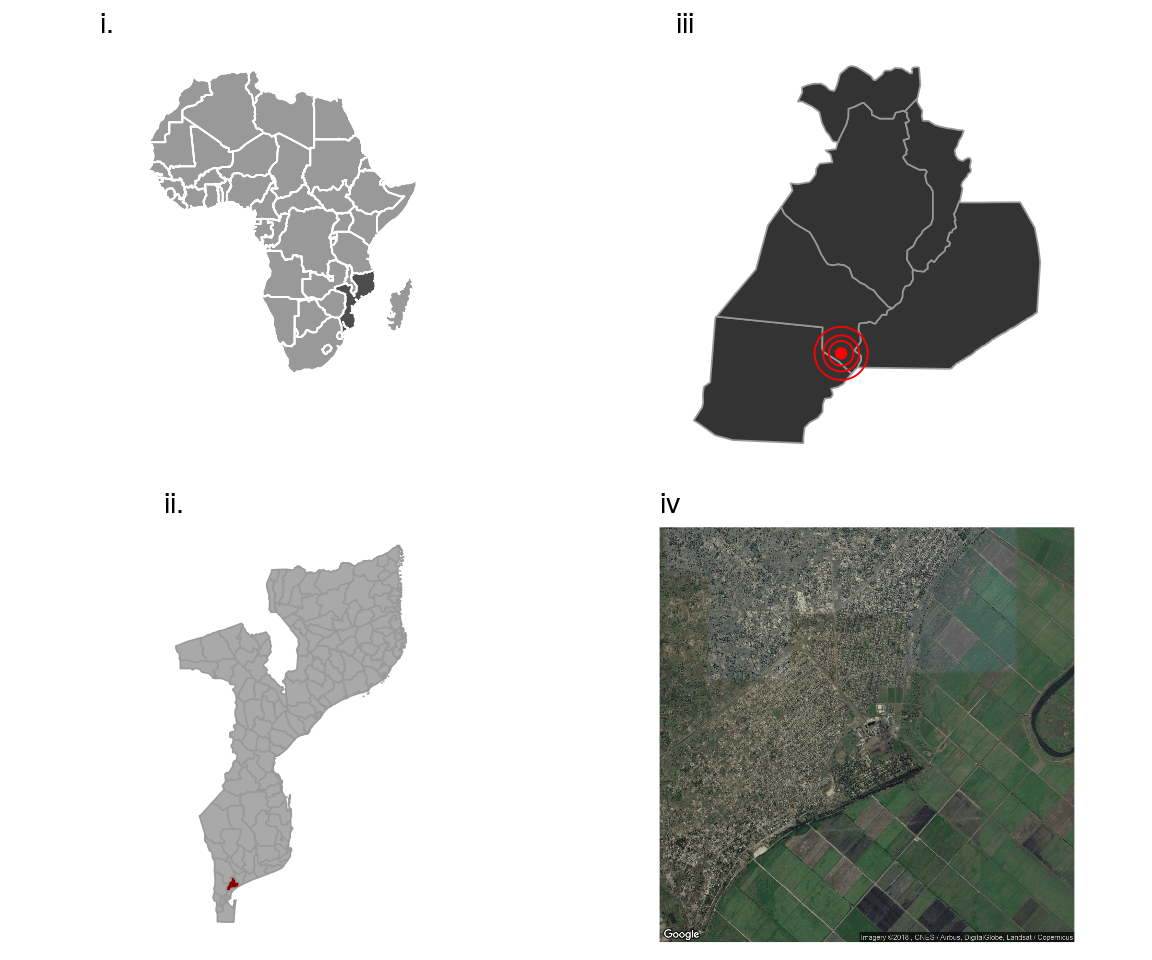
\includegraphics{menno_models_files/figure-latex/unnamed-chunk-14-1} \end{center}

\subsection{Model C (with seasonality and herd
score)}\label{model-c-with-seasonality-and-herd-score}

We now introduce herd immunity to the model. This is introduced as an
additive effect; perhaps it should be interactive with IRS? Using this
approach, our panel data looks like this:

\begin{verbatim}
# A tibble: 6 x 8
  oracle_number group       year_month absent  days  herd months_since_me~
  <chr>         <chr>       <chr>       <dbl> <int> <dbl> <fct>           
1 PF02492       Permanent ~ 2013_3       9.68    31 136   01              
2 X034289       Temporary ~ 2016_9       0       30 276   02              
3 PF00699       Permanent ~ 2016_9       0       30 282   03              
4 X044684       Temporary ~ 2014_9       0       30 248   01              
5 X045133       Temporary ~ 2015_8       6.45    31 156   06              
6 X041009       Temporary ~ 2015_6       0       30  97.1 02              
# ... with 1 more variable: season <fct>
\end{verbatim}

Our new model specification (in R) is:

\begin{verbatim}
felm(formula = absent ~ months_since_menno * season | oracle_number + 
    year_month | 0 | 0, data = these_data)
\end{verbatim}

The results of this model look like this:

\begin{longtable}[t]{ll}
\caption{\label{tab:unnamed-chunk-17}Simple models with year-month fixed effects, seasonality-IRS interaction term, and herd score}\\
\toprule
Term & Estimate\\
\midrule
\endfirsthead
\caption[]{Simple models with year-month fixed effects, seasonality-IRS interaction term, and herd score \textit{(continued)}}\\
\toprule
Term & Estimate\\
\midrule
\endhead
\
\endfoot
\bottomrule
\endlastfoot
\addlinespace[1.5em]
\multicolumn{2}{l}{\textbf{Permanent field worker}}\\
\hspace{1em}IRS status=\_menno01 & 175.053 (P=0.532)\\
\hspace{1em}IRS status=\_menno02 & 457.807 (P=0.115)\\
\hspace{1em}IRS status=\_menno03 & 505.425 (P=0.061)\\
\hspace{1em}IRS status=\_menno04 & 233.373 (P=0.357)\\
\hspace{1em}IRS status=\_menno05 & 227.399 (P=0.372)\\
\hspace{1em}IRS status=\_menno06 & 425.265 (P=0.121)\\
\hspace{1em}Malaria season & 887.601 (P=0.703)\\
\hspace{1em}IRS status=\_menno01:Malaria season & -58.338 (P=0.872)\\
\hspace{1em}IRS status=\_menno02:Malaria season & -174.777 (P=0.642)\\
\hspace{1em}IRS status=\_menno03:Malaria season & -603.926 (P=0.105)\\
\hspace{1em}IRS status=\_menno04:Malaria season & -220.413 (P=0.56)\\
\hspace{1em}IRS status=\_menno05:Malaria season & -213.141 (P=0.582)\\
\hspace{1em}IRS status=\_menno06:Malaria season & -191.654 (P=0.633)\\
\addlinespace[1.5em]
\multicolumn{2}{l}{\textbf{Permanent not field worker}}\\
\hspace{1em}IRS status=\_menno01 & 39.635 (P=0.788)\\
\hspace{1em}IRS status=\_menno02 & 14.833 (P=0.919)\\
\hspace{1em}IRS status=\_menno03 & 114.878 (P=0.439)\\
\hspace{1em}IRS status=\_menno04 & 55.896 (P=0.694)\\
\hspace{1em}IRS status=\_menno05 & 93.301 (P=0.502)\\
\hspace{1em}IRS status=\_menno06 & 86.299 (P=0.556)\\
\hspace{1em}Malaria season & NaN (PNA)\\
\hspace{1em}IRS status=\_menno01:Malaria season & -72.876 (P=0.707)\\
\hspace{1em}IRS status=\_menno02:Malaria season & 23.995 (P=0.903)\\
\hspace{1em}IRS status=\_menno03:Malaria season & 127.34 (P=0.523)\\
\hspace{1em}IRS status=\_menno04:Malaria season & -296.411 (P=0.137)\\
\hspace{1em}IRS status=\_menno05:Malaria season & -185.639 (P=0.372)\\
\hspace{1em}IRS status=\_menno06:Malaria season & -171.932 (P=0.416)\\
\addlinespace[1.5em]
\multicolumn{2}{l}{\textbf{Temporary field worker}}\\
\hspace{1em}IRS status=\_menno01 & -35.174 (P=0.339)\\
\hspace{1em}IRS status=\_menno02 & -6.152 (P=0.869)\\
\hspace{1em}IRS status=\_menno03 & -12.472 (P=0.732)\\
\hspace{1em}IRS status=\_menno04 & 18.095 (P=0.611)\\
\hspace{1em}IRS status=\_menno05 & 33.497 (P=0.346)\\
\hspace{1em}IRS status=\_menno06 & 9.614 (P=0.816)\\
\hspace{1em}Malaria season & 44.327 (P=0.309)\\
\hspace{1em}IRS status=\_menno01:Malaria season & 8.557 (P=0.881)\\
\hspace{1em}IRS status=\_menno02:Malaria season & 3.8 (P=0.948)\\
\hspace{1em}IRS status=\_menno03:Malaria season & -75.835 (P=0.21)\\
\hspace{1em}IRS status=\_menno04:Malaria season & -51.282 (P=0.397)\\
\hspace{1em}IRS status=\_menno05:Malaria season & -70.353 (P=0.217)\\
\hspace{1em}IRS status=\_menno06:Malaria season & 63.717 (P=0.259)\\
\addlinespace[1.5em]
\multicolumn{2}{l}{\textbf{Temporary not field worker}}\\
\hspace{1em}IRS status=\_menno01 & 414.405 (P=0.319)\\
\hspace{1em}IRS status=\_menno02 & 90.379 (P=0.825)\\
\hspace{1em}IRS status=\_menno03 & 353.397 (P=0.441)\\
\hspace{1em}IRS status=\_menno04 & -565.881 (P=0.232)\\
\hspace{1em}IRS status=\_menno05 & -355.43 (P=0.388)\\
\hspace{1em}IRS status=\_menno06 & 45.199 (P=0.895)\\
\hspace{1em}Malaria season & -459.147 (P=0.519)\\
\hspace{1em}IRS status=\_menno01:Malaria season & -724.867 (P=0.206)\\
\hspace{1em}IRS status=\_menno02:Malaria season & 661.492 (P=0.283)\\
\hspace{1em}IRS status=\_menno03:Malaria season & -1223.913 (P=0.031)\\
\hspace{1em}IRS status=\_menno04:Malaria season & 529.98 (P=0.364)\\
\hspace{1em}IRS status=\_menno05:Malaria season & 324.283 (P=0.578)\\
\hspace{1em}IRS status=\_menno06:Malaria season & 817.731 (P=0.227)\\*
\end{longtable}


\end{document}
